\documentclass[margin=2mm]{standalone}
\usepackage{tikz}
\usetikzlibrary{arrows.meta}
\begin{document}
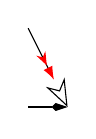
\begin{tikzpicture}-{Hooks[]}

\iffalse
->：这是最基本的箭头样式，表示一个简单的单向箭头。
-{>>>}：这个样式绘制了一个带有三个大尖头的箭头。
-{>[]>>}：这个样式绘制了一个带有方括号头部的箭头，箭头尾部是一个普通的线段。
-{>[]>[]>[]}：这个样式绘制了一个由方括号和尖头组成的复杂箭头。
-___>：这个样式绘制了一个带有横线头部的箭头，横线在箭头尖端之前延伸。
<.<->.>：这个样式绘制了一个双向箭头，箭头头部和尾部都是尖的。
-{Arc Barb[]}：这个样式绘制了一个带有弧形头部的箭头。
-{Bar[]}：这个样式绘制了一个带有平直条头的箭头。
-{Hooks[]}：这个样式绘制了一个带有钩形头部的箭头。
-{Parenthesis[]}：这个样式绘制了一个带有括号形状头部的箭头。
-{Straight Barb[]}：这个样式绘制了一个带有直线条头的箭头。
-{Tee Barb[]}：这个样式绘制了一个带有T形条头的箭头。
-{Classical TikZ Rightarrow[]}：这个样式绘制了一个类似于传统TikZ的右箭头。
-{Computer Modern Rightarrow[]}：这个样式绘制了一个类似于Computer Modern字体的右箭头。
-{Implies[] To[] Circle[]}：这个样式绘制了一个由蕴含箭头、到箭头和圆圈头组成的复合箭头。
-{Diamond[]}：这个样式绘制了一个带有菱形头部的箭头。
-{Ellipse[]}：这个样式绘制了一个带有椭圆形头部的箭头。
-{Kite[]}：这个样式绘制了一个带有风筝形状头部的箭头。
-{Latex[]}：这个样式绘制了一个带有LaTeX标志样式的箭头。
-{Rectangle[]}：这个样式绘制了一个带有矩形头部的箭头。
-{Square[]}：这个样式绘制了一个带有正方形头部的箭头。
-{Stealth[]}：这个样式绘制了一个带有尖锐箭头头部的箭头。
-{Triangle[]}：这个样式绘制了一个带有三角形头部的箭头。
-{Turned Square[]}：这个样式绘制了一个带有倒置的正方形头部的箭头。
-{Butt Cap[] Fast Round[]}：这个样式绘制了一个带有平直头部和快速圆形头部的箭头。
-{Fast Triangle[]}：这个样式绘制了一个带有快速三角形头部的箭头。
-{Round Cap[]}：这个样式绘制了一个带有圆形头部的箭头。
-{Triangle Cap[]}：这个样式绘制了一个带有三角形头部的箭头。
-{Rays[]}：这个样式绘制了一个带有射线形状头部的箭头。
\fi


\draw [-{Kite[]}] (0,0) -- (0.5,0);



 \tikzset{
    foo /.tip = {Stealth[sep] Latex[sep]},
    bar /.tip = {Stealth[length=10pt,open]}
}
\draw [-{foo[red] . bar}] (0,1) -- (0.5,0);
\end{tikzpicture}

\end{document}